\chapter{Interfaces con Android Studio}

A la hora de crear interfaces para dispositivos Android a través de Android Studio estos son generados a través de ficheros \href{https://es.wikipedia.org/wiki/Extensible_Markup_Language}{XML}. Para el correcto funcionamiento y compilación del proyecto, estos ficheros deben de cumplir con el estándar XML y ser ficheros válidos.

\errorbox{\textbf{¡Cuidado a la hora de tocar los ficheros si los editamos a mano!}}

Estos ficheros se encuentran por defecto en la ruta \configdir{src/main/res/layout} de nuestro proyecto. No es habitual editar estos ficheros fuera de Android Studio, pero hay que tener en cuenta dónde se almacenan.

\section{Creando nuestro primer proyecto}

Una vez abierto Android Studio vamos a crear un nuevo proyecto y vamos a elegir “Empty Views Activity”, de esta manera el proyecto que nos va a generar va a tener una primera vista con un texto centrado

\begin{center}
    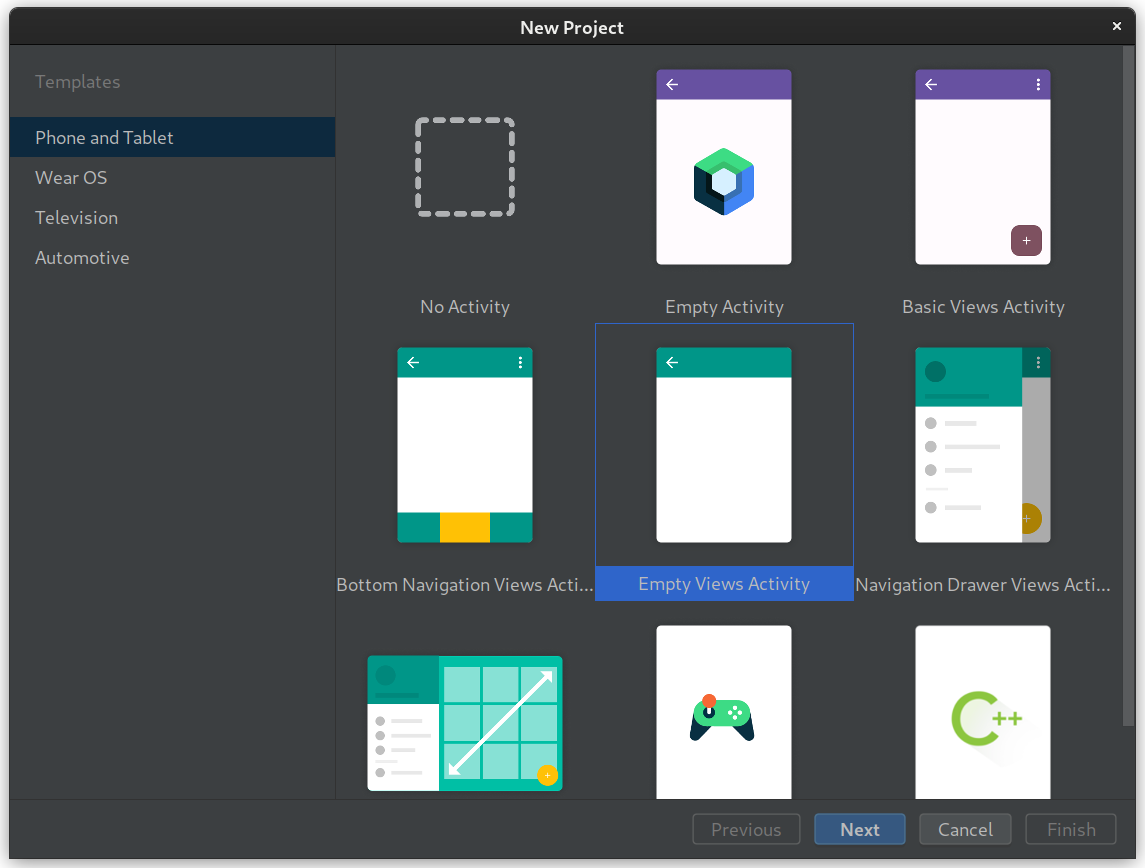
\includegraphics[width=0.4\linewidth]{crear_proyecto.png}
\end{center}